\documentclass[aspectratio=169]{beamer}
\usepackage[ngerman]{babel}
\usepackage[utf8]{inputenc}
\usepackage[T1]{fontenc}
\usepackage{lmodern}
\usepackage{listings}
\usepackage{xcolor}
\usepackage{apacite}
\usepackage[percent]{overpic}


\bibliographystyle{apacite}


\definecolor{codegreen}{rgb}{0,0.6,0}
\definecolor{codegray}{rgb}{0.5,0.5,0.5}
\definecolor{codepurple}{rgb}{0.58,0,0.82}
\definecolor{backcolour}{rgb}{0.95,0.95,0.92}
\definecolor{TUCgreen}{cmyk}{1,0,0.9,0.2}

\lstdefinestyle{mystyle}{
    backgroundcolor=\color{backcolour},   
    commentstyle=\color{codegreen},
    keywordstyle=\color{magenta},
    numberstyle=\tiny\color{codegray},
    stringstyle=\color{codepurple},
    basicstyle=\ttfamily\footnotesize,
    breakatwhitespace=false,         
    breaklines=true,                 
    captionpos=b,                    
    keepspaces=true,                 
    numbers=left,                    
    numbersep=5pt,                  
    showspaces=false,                
    showstringspaces=false,
    showtabs=false,                  
    tabsize=2
}

\lstset{style=mystyle}

\graphicspath{{figs/}}

    \usetheme{TUC2}
  %  \usefonttheme{structureitalicserif}
    \setbeamercovered{transparent}
\newcommand{\FEsq}{FE$^2\,$}

\mode<presentation>
    \title{Neural Network-based Detection of Taylor Vortices in Annular Flow Systems}
    \subtitle{Exposé for Master Thesis - Initial Presentation}
    \author{\textbf{Mahyar Alikhani}}
    \institute{Institute of Applied Mechanics}
    \date{\today}

% \setbeamerfont{framesubtitle}{size=\normalfont\tiny}
%%%%%%%%%%%%%%%%%%%%%%%%%%%%%%%%%%%%%%%%%%%%%%%%%%%%%%
\begin{document}
\begin{frame}
\titlepage
% Collaborators: \footnotesize{
%   Stefan Wittek$^1$, Jendrik-Alexander Tr\"oger$^2$, Stefan Hartmann$^2$, Andreas Rausch$^1$
%      }
\end{frame}
%%%%%%%%%%%%%%%%%%%%%%%%%%%%%%%%%%%%%%%%%%%%%%%%%%%%%%

\begin{frame}
\frametitle{Contents}
\tableofcontents
\end{frame}

%%%%%%%%%%%%%%%%%%%%%%%%%%%%%%%%%%%%%%%%%%%%%%%%%%%%%%
\section{Problem Statment}
\begin{frame}
  \frametitle{Problem Statment}
  \large \color{TUCgreen}\textbf{Taylor-coutte Flow}
  \begin{itemize}
    \item is defined as a fluid dynamic phenomenon that occurs when a fluid is passing between two coaxial-rotating cylinders.
    \item 
  \end{itemize}
\end{frame}

%%%%%%%%%%%%%%%%%%%%%%%%%%%%%%%%%%%%%%%%%%%%%%%%%%%%%%
\section{Task definition and objective}
\begin{frame}
  \frametitle{Objectives}
\end{frame}


%%%%%%%%%%%%%%%%%%%%%%%%%%%%%%%%%%%%%%%%%%%%%%%%%%%%%%
\section{Approache}
\begin{frame}
  \frametitle{Approaches}
\end{frame}
%%%%%%%%%%%%%%%%%%%%%%%%%%%%%%%%%%%%%%%%%%%%%%%%%%%%%%
\section{Initial Results}
\begin{frame}
  \frametitle{Results}
\end{frame}

%%%%%%%%%%%%%%%%%%%%%%%%%%%%%%%%%%%%%%%%%%%%%%%%%%%%%%
\begin{frame}
\frametitle{}\
  \begin{minipage}{0.45\textwidth}
    \centering
    %(A) Global ---> Global
    \vfill
    %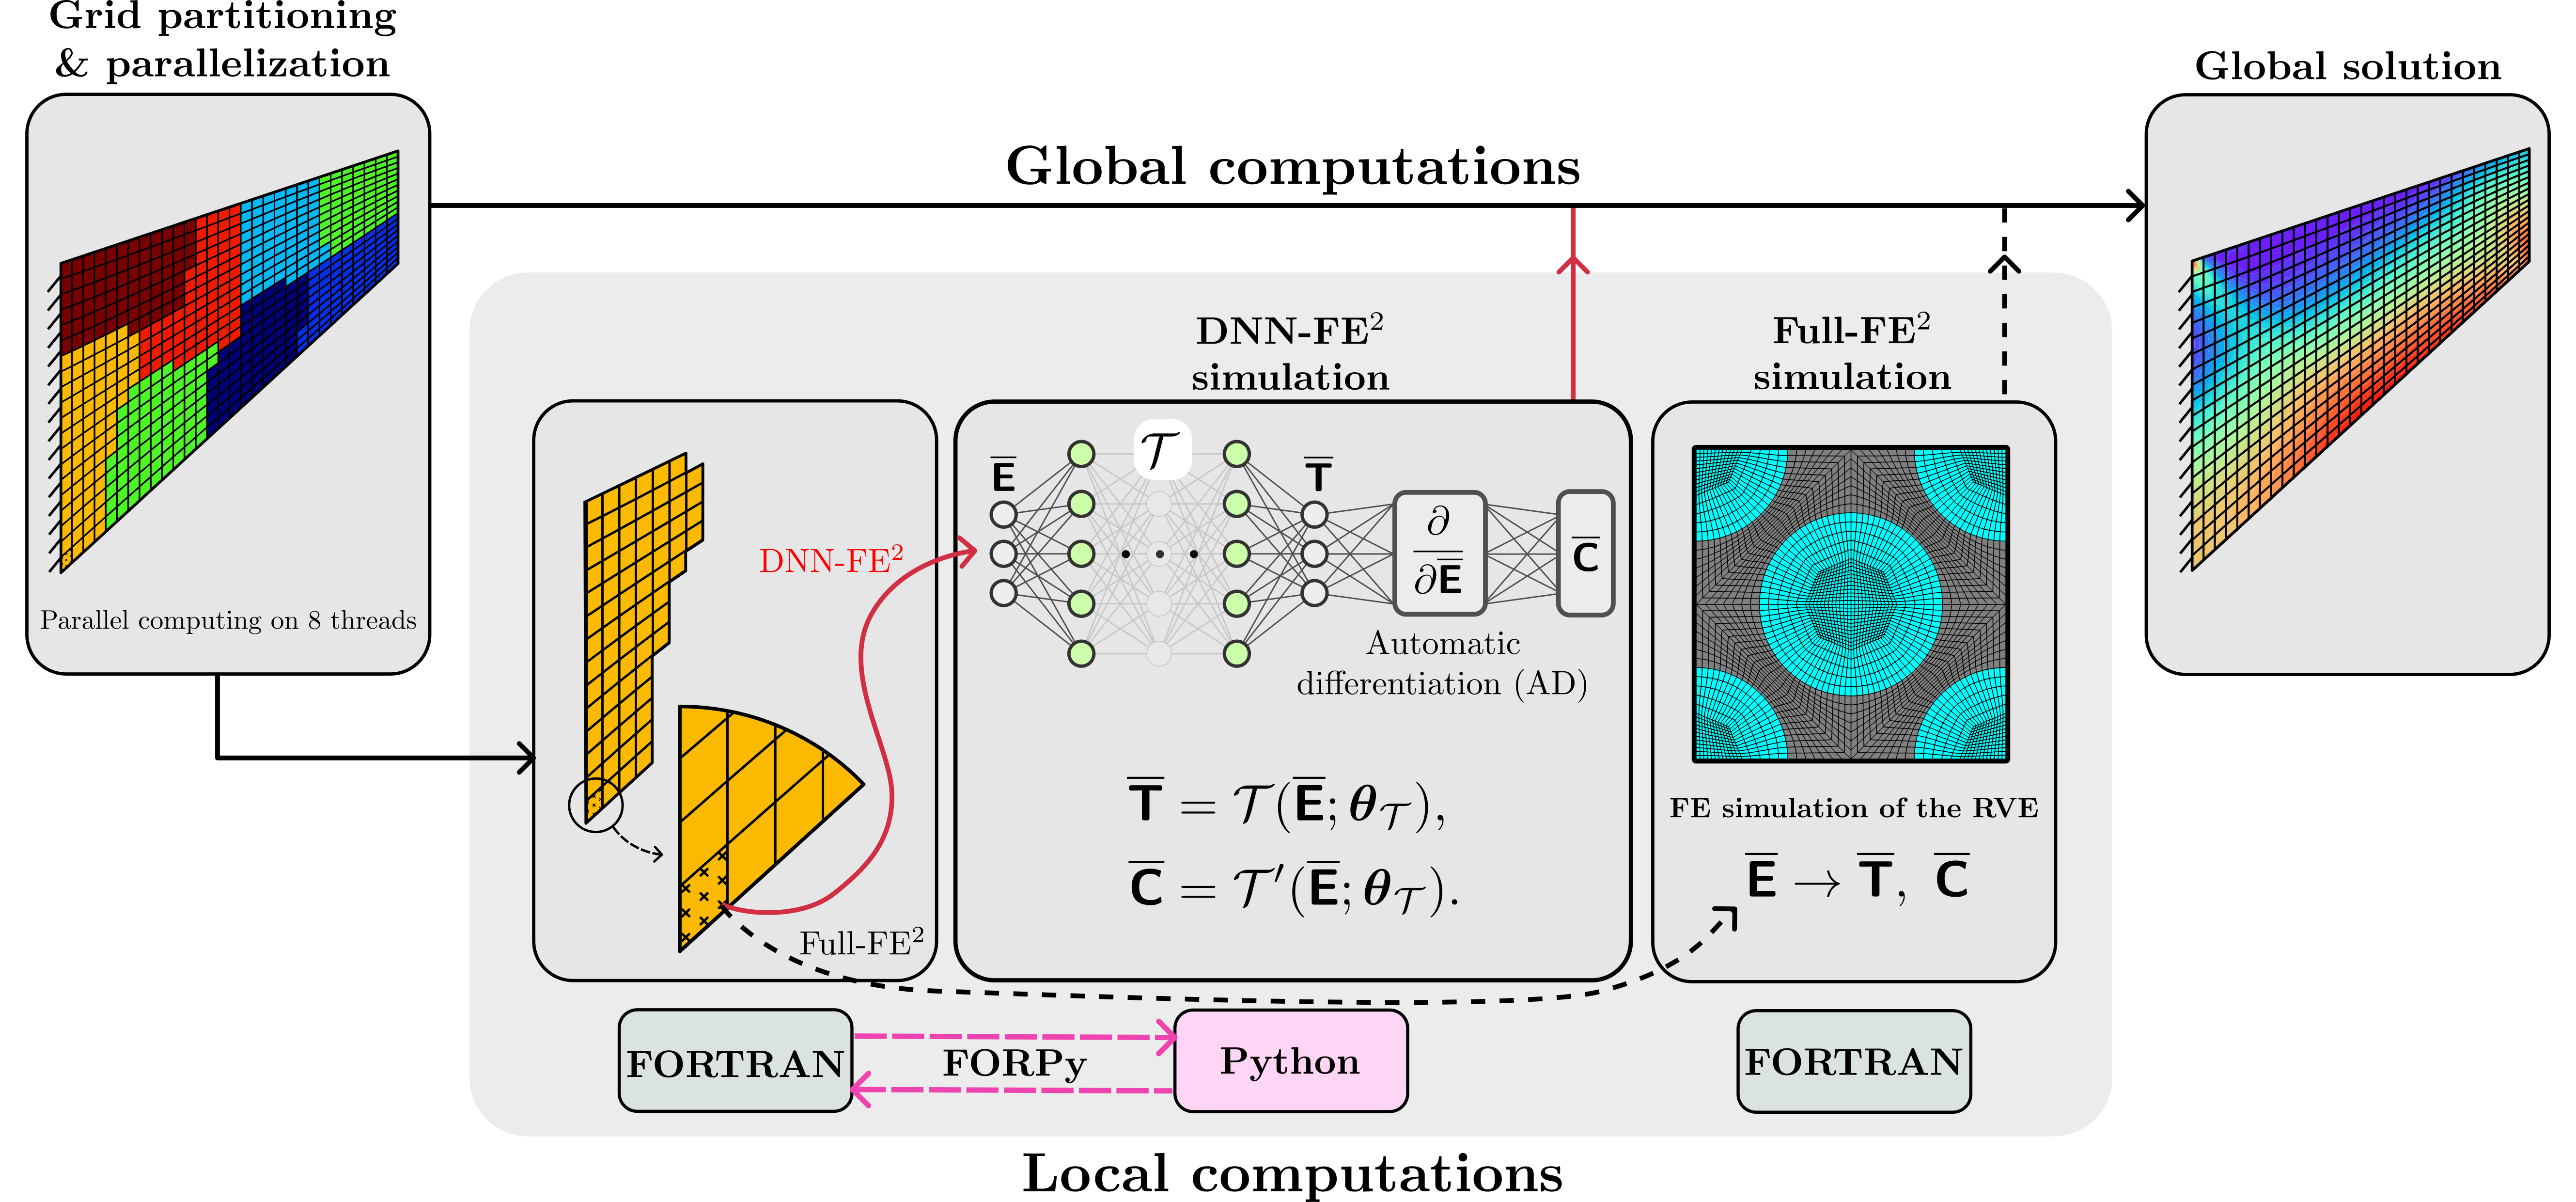
\includegraphics[width=0.9\textwidth, trim={10cm 2.3cm 9.9cm 4.2cm}, clip]{drawing}
  \end{minipage}
  \begin{minipage}{0.45\textwidth}
    \centering
    %(B) Global ---> Local ---> Global
    \vfill
    %\hfill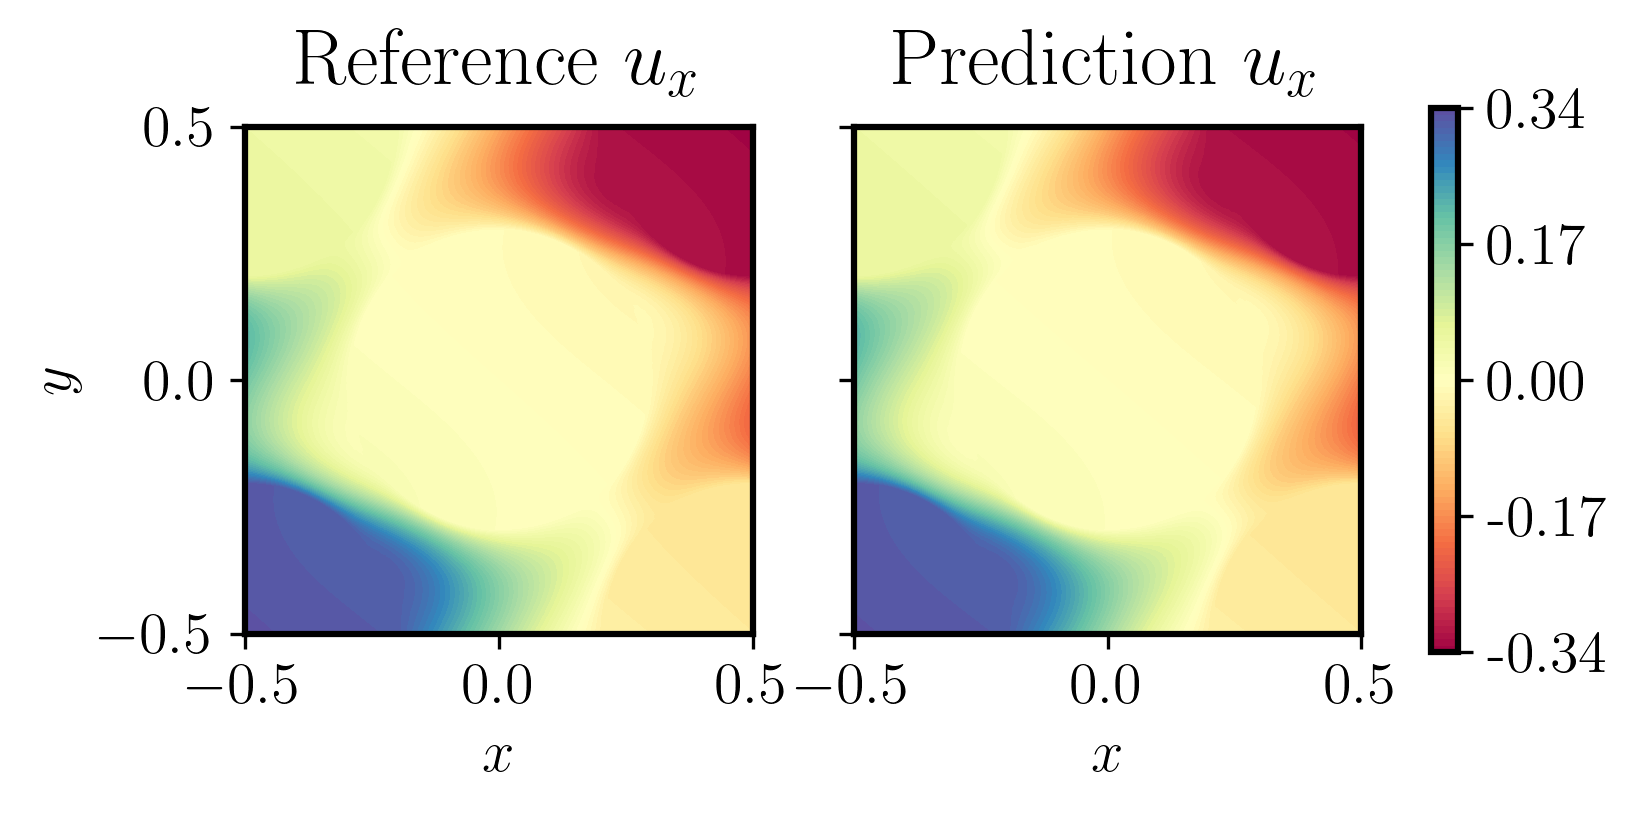
\includegraphics[width=0.95\textwidth, trim={0cm 0cm 7cm 0cm}, clip]{rve1_ux.png}
  \end{minipage}
\end{frame}


%%%%%%%%%%%%%%%%%%%%%%%%%%%%%%%%%%%%%%%%%%%%%%%%%%%%%%

\begin{frame}
  \frametitle{}\
  
\begin{minipage}{0.3\textwidth}
    %Inputs of branch: \\$\mathbf{E} \in \mathbb{R}^3$, ($N_s$, 3)

    %Outputs of branch: \\$\boldsymbol{b} \in \mathbb{R}^{N_f}$, ($N_s$, $N_f$)

    \vspace{\baselineskip}

    %Inputs of trunk: \\$\mathbf{X} \in \mathbb{R}^{10561}$, (10561, 2)

    %Outputs of trunk: \\$\boldsymbol{t} \in \mathbb{R}^{N_f}$, (10561, $N_f$)
\end{minipage}
\begin{minipage}{0.35\textwidth}
    %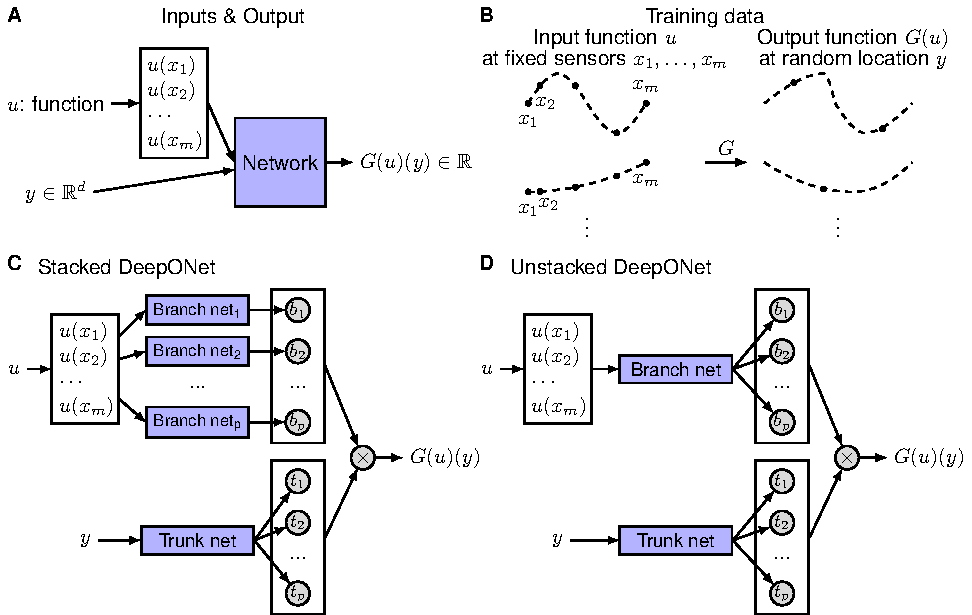
\includegraphics[width=\textwidth, trim={10.05cm 0cm 0cm 4.8cm}, clip]{deeponet.pdf}
\end{minipage}
\begin{minipage}{0.3\textwidth}

  %Outputs: \\$\boldsymbol{u} \in \mathbb{R}^{2\times10561}$, \\($N_s$, $N_f$) $\bigotimes$ (10561, $N_f$)$^{T}$

\end{minipage}
\end{frame}


\section{Time Planning}
\begin{frame}
  \frametitle{Timeline}
  \begin{center}
    \begin{figure}
      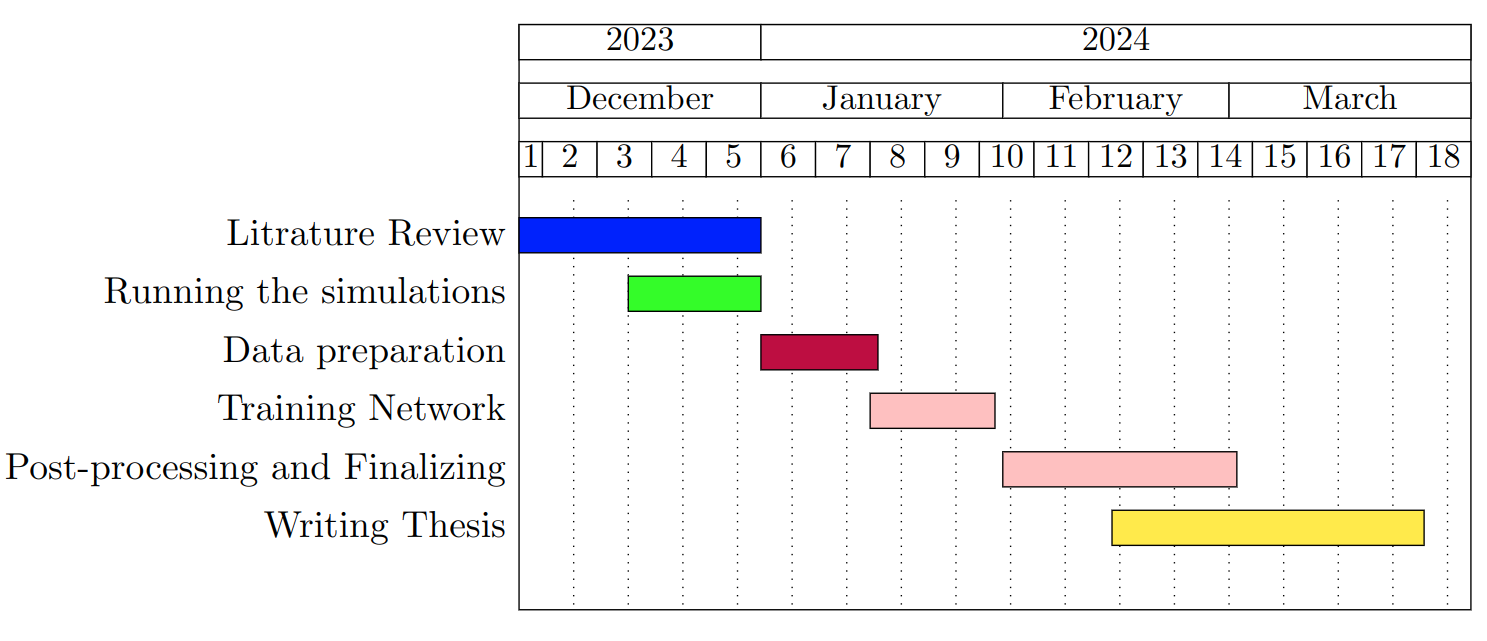
\includegraphics[width=0.9\textwidth]{figs/Timeplan.png}
      \caption{Timeplan}
    \end{figure}
  \end{center} 
\end{frame}

\begin{frame}
  % \centering
  \begin{minipage}{0.1\textwidth}
    \hfill
  \end{minipage}
  \begin{minipage}{0.89\textwidth}
    \color{TUCgreen}{\textbf{\Large{Thank you!}}}\\
  \color{black}{
  \small{Any questions?}
  }
  \end{minipage}
  
\end{frame}

\end{document}

